\documentclass{standalone}
\usepackage{graphicx}	
\usepackage{amssymb, amsmath}
\usepackage{color}

\usepackage{tikz}
\usetikzlibrary{shapes}
\usepackage{pgfmath}

\definecolor{light}{RGB}{220, 188, 188}
\definecolor{mid}{RGB}{185, 124, 124}
\definecolor{dark}{RGB}{143, 39, 39}
\definecolor{highlight}{RGB}{180, 31, 180}
\definecolor{gray10}{gray}{0.1}
\definecolor{gray20}{gray}{0.2}
\definecolor{gray30}{gray}{0.3}
\definecolor{gray40}{gray}{0.4}
\definecolor{gray60}{gray}{0.6}
\definecolor{gray70}{gray}{0.7}
\definecolor{gray80}{gray}{0.8}
\definecolor{gray90}{gray}{0.9}
\definecolor{gray95}{gray}{0.95}

\newcommand*{\offset}{0.025}

\begin{document}

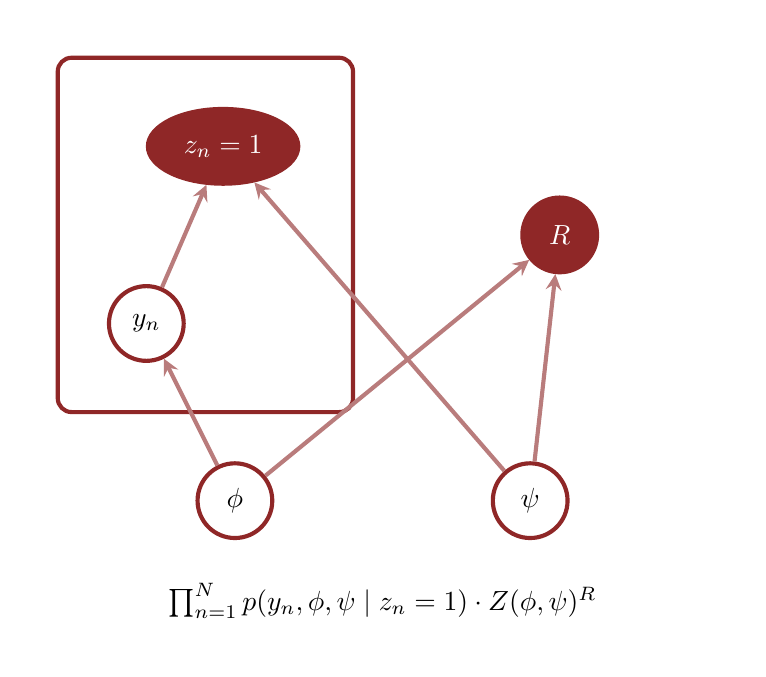
\begin{tikzpicture}[
   scale=0.2,
   obscirc/.style={circle, draw=dark, fill=dark, line width=1.5, text=white,
               inner sep=5, minimum size=27},
   obsell/.style={ellipse, draw=dark, fill=dark, line width=1.5, text=white,
                  inner sep=5, minimum height=27},
   unobscirc/.style={circle, draw=dark, fill=white, line width=1.5, text=black,
                     inner sep=5, minimum size=27},
   unobsell/.style={ellipse, draw=dark, fill=white, line width=1.5, text=black,
                    inner sep=5, minimum height=27}
  ]

  % Node Spacing
  \pgfmathsetmacro{\d}{7.5}
  
  \begin{scope}[shift={(0, 0)}]
    \draw[white] (-3 * \d, -1.25 * \d) rectangle (3 * \d, 4 * \d);
  
    \draw[dark, line width=1.5, rounded corners=5] (-0.25 * \d, 0.75 * \d) rectangle (-2.75 * \d, 3.75 * \d);
 
    \node (A) at (-1.25 * \d, 0) [unobscirc] { $\phi$ };
    \node (B) at (+1.25 * \d, 0) [unobscirc] { $\psi$ };
    
    \node (C) at (-2 * \d, 1.5 * \d) [unobscirc] { $y_{n}$ };
    \node (D) at (-1.35 * \d, 3 * \d) [obsell] { $z_{n} = 1$ };

    \node (F) at (+1.5 * \d, 2.25 * \d) [obscirc] { $R$ };

    \foreach \B/\E in {A/C, B/D, C/D, A/F, B/F} {
      \draw[->, >=stealth, color=mid, line width=1.5] (\B) -- (\E);
    }
    
    \node at (0, -0.85 * \d) { $      \prod_{n = 1}^{N} p(y_{n}, \phi, \psi \mid z_{n} = 1)
                                \cdot Z(\phi, \psi)^{R}$ };

  \end{scope}

\end{tikzpicture}

\end{document}  